
%(BEGIN_QUESTION)
% Copyright 2014, Tony R. Kuphaldt, released under the Creative Commons Attribution License (v 1.0)
% This means you may do almost anything with this work of mine, so long as you give me proper credit

{\it Complex numbers} are commonly used in AC circuit analysis to represent voltage, current, and impedance quantities.  A complex number is a quantity having both a ``real'' and an ``imaginary'' value, and may be represented as a vector on a complex plane.  For example, the following complex number has a ``real'' part equal to +4 and an ``imaginary'' part equal to +j3 (also written as +i3):

$$\includegraphics[width=15.5cm]{i03067x02.eps}$$

Complex numbers may be written in terms of their real and imaginary parts, in which case we refer to the notation as {\it rectangular}.  The complex number in the above illustration is $4 + j3$ in rectangular form.  Complex numbers may alternatively be written in terms of their magnitude and angle, in which case we refer to the notation as {\it polar}.  The complex number in the above illustration is $5 \> \angle \> 36.87^o$ in polar form.

\vskip 10pt

Your task is to build a computer spreadsheet program to convert from any complex number entered in rectangular form into polar form, or vice-versa.  A sample layout is presented here, where yellow shading represents values entered by you, and blue shading represents values calculated by the computer.  Two sets of cells are shown, one for converting rectangular to polar and another for converting polar to rectangular:

$$
\includegraphics[width=15.5cm]{i03067x01.eps}$$

\vskip 10pt

\filbreak

When you are finished entering your spreadsheet's formulae, test it by converting between the following complex number formats:

\begin{itemize}
\item{} $56 - j23$ = 
\vskip 10pt
\item{} $105 \> \angle \> 20^o$ = 
\vskip 10pt
\item{} $15304 \> \angle \> 175^o$ = 
\vskip 10pt
\item{} $-930 + j12944$ = 
\end{itemize}

Note: you are going to need a way to quickly convert between rectangular and polar forms of complex numbers with some of the AC circuit calculations in this course!

\vskip 20pt

An alternative to building a spreadsheet is to familiarize yourself with your scientific calculator's complex number functions, if it offers this functionality.  If you have such a calculator, you may practice the following calculations in lieu of building the spreadsheet:

\begin{itemize}
\item{} $(-15 + j4) + (32 - j12) = $
\vskip 10pt
\item{} $(24 - j18) \times (3 + j9) = $
\vskip 10pt
\item{} $(35 \angle 40^o) \times (8 \angle 130^o) = $
\vskip 10pt
\item{} $(10 - j25) \div (19 \angle 31^o) = $
\vskip 10pt
\item{} $(43 \angle 80^o) + (35 \angle -15^o) = $
\end{itemize}

\underbar{file i03067}
%(END_QUESTION)





%(BEGIN_ANSWER)

\begin{itemize}
\item{} $56 - j23$ = $60.54 \> \angle \> -22.33^o$ 
\vskip 10pt
\item{} $105 \> \angle \> 20^o$ = $98.67 + j35.91$
\vskip 10pt
\item{} $15304 \> \angle \> 175^o$ = $-15245.8 + j1333.8$
\vskip 10pt
\item{} $-930 + j12944$ = $12977.4 \> \angle \> 94.11^o$
\end{itemize}

%(END_ANSWER)





%(BEGIN_NOTES)

\noindent
Calculator practice:

\begin{itemize}
\item{} $(-15 + j4) + (32 - j12) = 17 - j8$
\vskip 10pt
\item{} $(24 - j18) \times (3 + j9) = 234 + j162$
\vskip 10pt
\item{} $(35 \angle 40^o) \times (8 \angle 130^o) = 280 \angle 170^o$
\vskip 10pt
\item{} $(10 - j25) \div (19 \angle 31^o) = -0.2265 - j1.3989 = 1.4171 \angle 260.8^o$
\vskip 10pt
\item{} $(43 \angle 80^o) + (35 \angle -15^o) = 53.025 \angle 38.886^o$
\end{itemize}


%INDEX% Computer spreadsheet exercise: polar/rectangular complex number converter

%(END_NOTES)


